\newpage
\section{Các yêu cầu chức năng}

Dự án được chia làm 5 phân hệ (5 Use-case lớn), mỗi phân hệ được một thành viên nhóm đảm nhiệm.

\subsection{Use-case diagram cho toàn bộ hệ thống}
\begin{figure}[H]
    \centering
    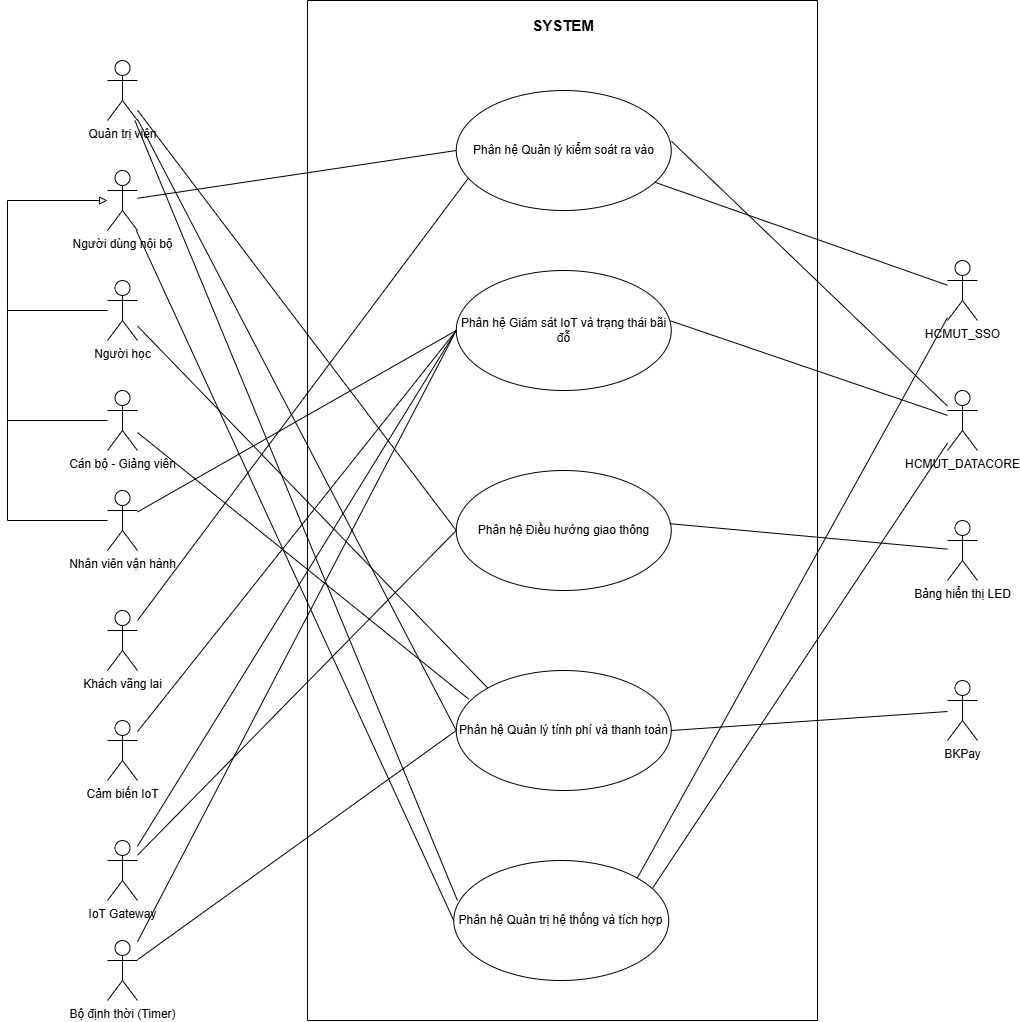
\includegraphics[width=1.1\textwidth]{pictures/whole_system_UCD.drawio.png} 
    \caption{Use-case diagram cho toàn hệ thống}
    \label{UCD_All}
\end{figure}

\subsection{Quản trị Hệ thống và Tích hợp}
\subsubsection{Tổng quan}
Phân hệ này cho phép người dùng (sinh viên, cán bộ, giảng viên và quản trị viên) đăng nhập an toàn vào hệ thống IoT-SPMS thông qua cổng HCMUT\_SSO. Sau khi xác thực, hệ thống sẽ đồng bộ dữ liệu cá nhân từ HCMUT\_DATACORE để thiết lập phân quyền truy cập (RBAC), đồng thời hỗ trợ quản trị viên truy vết lịch sử hoạt động và xuất báo cáo. Điều này đảm bảo việc quản lý hệ thống được tập trung, bảo mật và luôn đồng nhất với cơ sở dữ liệu chính thức của nhà trường.

\subsubsection{Use-case diagram}
\begin{figure}[H]
    \centering
    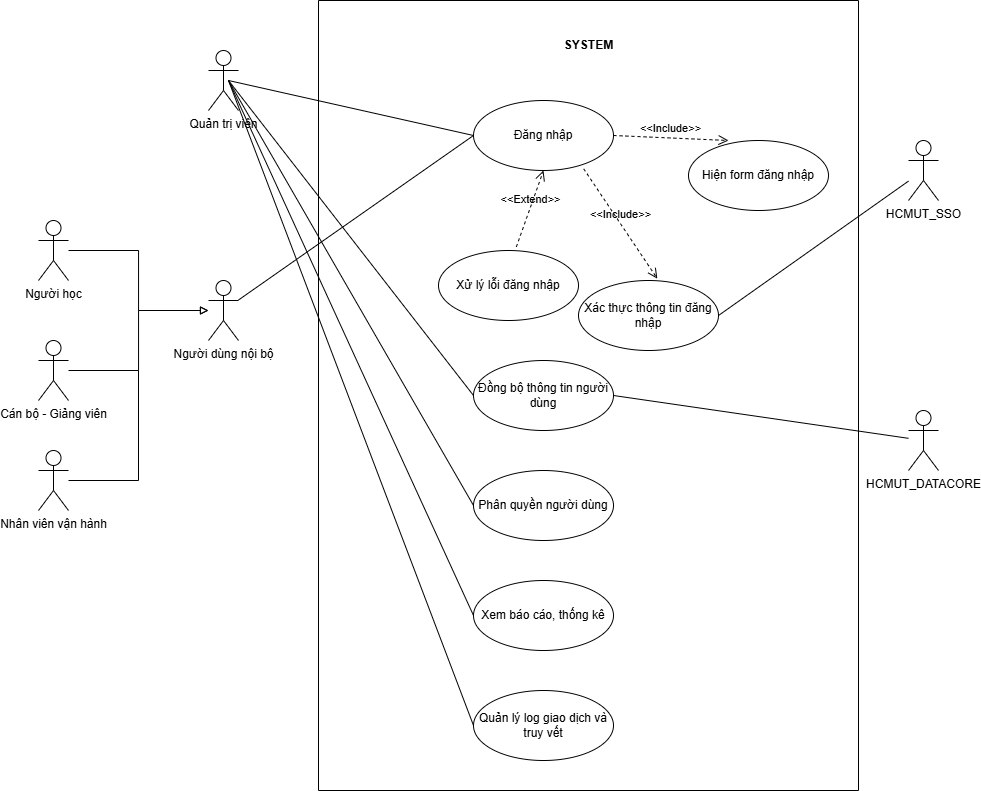
\includegraphics[width=1.1\textwidth]{pictures/UCD_Task5.png} 
    \caption{Use-case diagram cho Phân hệ Quản trị Hệ thống và Tích hợp}
    \label{UCD_Admin}
\end{figure}

\subsubsection{Use-case Scenarios}

\noindent \textbf{Use Case: Đăng nhập} \\
\renewcommand{\arraystretch}{1.6}
\begin{xltabular}{\textwidth}{|l|X|}
\hline
\textbf{Thuộc tính} & \textbf{Chi tiết} \\
\hline
\textbf{Tên} & Đăng nhập \\
\hline
\textbf{Tác nhân} & Người dùng nội bộ (Người học, Cán bộ - Giảng viên, Nhân viên vận hành), Quản trị viên \\
\hline
\textbf{Mô tả} & Cho phép người dùng đăng nhập và xác thực danh tính thông qua cổng HCMUT\_SSO để truy cập vào hệ thống bãi đỗ xe với các quyền hạn tương ứng. \\
\hline
\textbf{Tiền điều kiện} & Người dùng có tài khoản email HCMUT hợp lệ. Hệ thống có kết nối mạng để gọi sang HCMUT\_SSO. \\
\hline
\textbf{Luồng chính} & 
1. Người dùng truy cập vào trang chủ IoT-SPMS và nhấn nút "Đăng nhập". \newline
2. Hiện form đăng nhập. Hệ thống điều hướng người dùng sang trang hiển thị form đăng nhập chuẩn của trường. \newline
3. Người dùng nhập tên tài khoản, mật khẩu và nhấn "Login". \newline
4. Hệ thống nhận thông tin và gửi yêu cầu xác thực qua API của HCMUT\_SSO. \newline
5. HCMUT\_SSO trả về Token xác nhận đăng nhập thành công. \newline
6. Hệ thống giải mã Token, đối chiếu với cơ sở dữ liệu nội bộ để xác định vai trò (Role) của người dùng. \newline
7. Hệ thống thiết lập phiên làm việc (Session) và điều hướng vào giao diện tương ứng (VD: Quản trị viên vào trang Admin, Sinh viên vào trang xem vị trí đỗ).\\
\hline
\textbf{Luồng ngoại lệ} & 
\textbf{EF1: Sai thông tin tài khoản hoặc mật khẩu (Tại bước 5)} \newline
5.1. HCMUT\_SSO trả về trạng thái lỗi xác thực. \newline
5.2. Hệ thống hiển thị thông báo "Tài khoản hoặc mật khẩu không chính xác", yêu cầu người dùng nhập lại ở form đăng nhập hiện tại. Luồng quay lại Bước 3. \\
\hline
\textbf{Hậu điều kiện} & Người dùng đăng nhập thành công và được điều hướng đến màn hình chính (Dashboard) phù hợp với vai trò. \\
\hline
\end{xltabular}

\newpage
\noindent \textbf{Use Case: Đồng bộ thông tin người dùng} \\
\renewcommand{\arraystretch}{1.6}
\begin{xltabular}{\textwidth}{|l|X|}
\hline
\textbf{Thuộc tính} & \textbf{Chi tiết} \\
\hline
\textbf{Tên} & Đồng bộ thông tin người dùng \\
\hline
\textbf{Tác nhân} & Quản trị viên, HCMUT\_DATACORE \\
\hline
\textbf{Mô tả} & Quản trị viên thực hiện kéo dữ liệu cá nhân và vai trò người dùng (sinh viên, cán bộ...) từ hệ thống HCMUT\_DATACORE về cơ sở dữ liệu nội bộ của bãi xe. \\
\hline
\textbf{Tiền điều kiện} & Quản trị viên đã đăng nhập thành công. Hệ thống kết nối được với HCMUT\_DATACORE. \\
\hline
\textbf{Luồng chính} & 
1. Quản trị viên chọn mục "Đồng bộ dữ liệu" trên thanh menu và nhấn "Khởi chạy đồng bộ". \newline
2. Hệ thống thiết lập kết nối API an toàn đến HCMUT\_DATACORE. \newline
3. HCMUT\_DATACORE chấp nhận yêu cầu và trả về tập dữ liệu dưới định dạng "chỉ đọc" (read-only). \newline
4. Hệ thống quét tập dữ liệu trả về, tiến hành thêm mới các tài khoản chưa có và cập nhật thông tin các tài khoản đã tồn tại vào cơ sở dữ liệu của bãi xe. \newline
5. Hệ thống hiển thị thông báo "Đồng bộ thành công X tài khoản" và ghi nhận lịch sử vào log. \\
\hline
\textbf{Luồng ngoại lệ} & 
\textbf{EF1: Mất kết nối với DATACORE (Tại bước 2)} \newline
2.1. Hệ thống không thể gọi API thành công. \newline
2.2. Hệ thống hiển thị thông báo lỗi: "Không thể kết nối với máy chủ DATACORE. Vui lòng kiểm tra lại mạng hoặc thử lại sau". Luồng kết thúc. \\
\hline
\textbf{Hậu điều kiện} & Dữ liệu người dùng trong IoT-SPMS được cập nhật khớp với HCMUT\_DATACORE. \\
\hline
\end{xltabular}

\newpage
\noindent \textbf{Use Case: Phân quyền người dùng} \\
\renewcommand{\arraystretch}{1.6}
\begin{xltabular}{\textwidth}{|l|X|}
\hline
\textbf{Thuộc tính} & \textbf{Chi tiết} \\
\hline
\textbf{Tên} & Phân quyền người dùng \\
\hline
\textbf{Tác nhân} & Quản trị viên \\
\hline
\textbf{Mô tả} & Quản trị viên thiết lập hoặc thay đổi vai trò truy cập (Role-Based Access Control) cho người dùng, chẳng hạn như gán quyền "Nhân viên vận hành" cho một mã số cán bộ cụ thể. \\
\hline
\textbf{Tiền điều kiện} & Quản trị viên đã đăng nhập. Dữ liệu người dùng đã được đồng bộ từ DATACORE. \\
\hline
\textbf{Luồng chính} & 
1. Quản trị viên truy cập trang "Quản lý phân quyền". \newline
2. Hệ thống hiển thị danh sách người dùng và vai trò hiện tại. \newline
3. Quản trị viên tìm kiếm và chọn một người dùng cụ thể, sau đó gán vai trò mới từ danh sách (VD: Nhân viên vận hành) và nhấn "Lưu". \newline
4. Hệ thống xác thực tính hợp lệ, cập nhật quyền mới vào cơ sở dữ liệu nội bộ. \newline
5. Hệ thống báo thành công và ghi log thao tác thay đổi quyền. \\
\hline
\textbf{Luồng ngoại lệ} & 
\textbf{EF1: Hủy thao tác (Tại bước 3)} \newline
3.1. Quản trị viên nhấn "Hủy" thay vì "Lưu". \newline
3.2. Hệ thống đóng cửa sổ phân quyền, không lưu thay đổi và giữ nguyên giao diện danh sách. \\
\hline
\textbf{Hậu điều kiện} & Quyền hạn của người dùng được cập nhật mới trên hệ thống. \\
\hline
\end{xltabular}

\newpage
\subsection{Quản lý kiểm soát ra vào}

\subsubsection{Tổng quan}
Phân hệ này cho phép quản lý tự động quy trình ra vào bãi đỗ xe cho cả người dùng nội bộ (thông qua thẻ định danh tích hợp) và khách vãng lai (thông qua vé tạm thời). Khi phương tiện qua cổng, hệ thống sẽ tiến hành xác thực danh tính, tự động điều khiển rào chắn (barrier) và ghi nhận thời gian của phiên đỗ xe, đồng thời cung cấp cơ chế vận hành ngoại tuyến để duy trì hoạt động ngay cả khi mất kết nối mạng. Điều này giúp giải quyết triệt để tình trạng ùn tắc tại các cổng kiểm soát, đảm bảo an ninh và cung cấp dữ liệu đầu vào chuẩn xác cho quá trình tính phí tự động.

\subsubsection{Use-case diagram}

\begin{figure}[H]
    \centering
    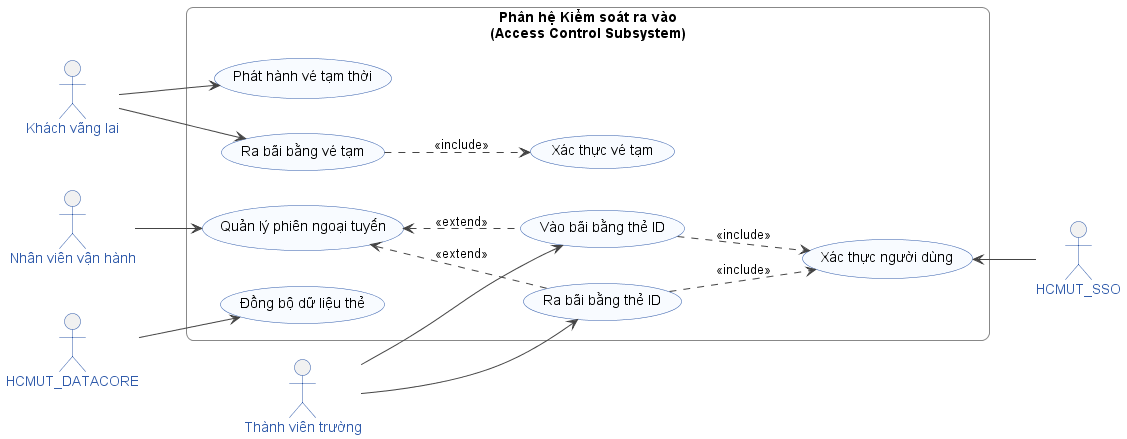
\includegraphics[width=1.1\textwidth]{pictures/task1_usecase_diagram.png} 
    \caption{Use-case diagram cho Phân hệ Quản lý kiểm soát ra vào}
    \label{UCD_1}
\end{figure}

\subsubsection{Use-case scenarios}

\noindent \textbf{Use Case: Vào bãi xe bằng thẻ ID} \\
\renewcommand{\arraystretch}{1.6}
\begin{xltabular}{\textwidth}{|l|X|}
\hline
\textbf{Thuộc tính} & \textbf{Chi tiết} \\
\hline
\textbf{Tên} & Vào bãi xe bằng thẻ ID \\
\hline
\textbf{Tác nhân} & Thành viên trường (Sinh viên, Cán bộ - Giảng viên,...) \\
\hline
\textbf{Mô tả} & Ghi nhận tự động lượt vào bãi xe của các thành viên chính thức sử dụng thẻ định danh. \\
\hline
\textbf{Tiền điều kiện} & Người dùng có thẻ định danh hợp lệ đã được đồng bộ từ HCMUT\_DATACORE. Bãi xe hiện tại chưa đạt trạng thái "Hết chỗ". \\
\hline
\textbf{Luồng chính} & 
1. Thành viên trường quẹt thẻ định danh tại đầu đọc (RFID/NFC) ở cổng vào. \newline
2. Hệ thống gửi yêu cầu xác thực thông tin thẻ qua nền tảng HCMUT\_SSO. \newline
3. HCMUT\_SSO trả về kết quả xác thực thành công.\newline
4. Camera tại cổng tự động chụp ảnh biển số và người điều khiển.\newline
5. Hệ thống khởi tạo một phiên gửi xe (parking session) mới lưu trữ: Mã thẻ, Biển số xe, Thời gian vào, Hình ảnh.\newline
6. Hệ thống kích hoạt relay mở barrier.\newline
7. Xe đi qua cổng; cảm biến (sensor) xác nhận và tự động đóng barrier.\newline
8. Hệ thống cập nhật giảm đi 1 chỗ trống trên dữ liệu bãi đỗ.\\
\hline
\textbf{Luồng ngoại lệ} & 
\textbf{Thẻ không hợp lệ/Chưa đăng ký}: Hệ thống báo lỗi bằng âm thanh/đèn LED, barrier không mở. Yêu cầu Member liên hệ Operator. \newline

\textbf{Bãi xe hết chỗ}: Đầu đọc thẻ bị vô hiệu hóa, màn hình LED hiển thị "Hết chỗ" và từ chối mở cổng.\\

\hline
\textbf{Hậu điều kiện} & Một phiên gửi xe mới được ghi nhận vào hệ thống. \\
\hline
\end{xltabular}

\noindent \textbf{Use Case: Rời bãi xe bằng thẻ ID} \\
\renewcommand{\arraystretch}{1.6}
\begin{xltabular}{\textwidth}{|l|X|}
\hline
\textbf{Thuộc tính} & \textbf{Chi tiết} \\
\hline
\textbf{Tên} & Rời bãi xe bằng thẻ ID \\
\hline
\textbf{Tác nhân} & Thành viên trường (Sinh viên, Cán bộ - Giảng viên,...) \\
\hline
\textbf{Mô tả} & Ghi nhận thời gian xe ra khỏi bãi thông qua thẻ định danh, tạo tiền đề cho việc tổng hợp tính phí. \\
\hline
\textbf{Tiền điều kiện} & Xe của thành viên trường đang ở trong bãi (có một phiên gửi xe đang hoạt động gắn với mã thẻ). \\
\hline
\textbf{Luồng chính} & 
1. Thành viên trường quẹt thẻ định danh tại đầu đọc ở cổng ra.

2. Hệ thống kiểm tra mã thẻ và truy xuất phiên gửi xe đang hoạt động tương ứng.

3. Camera cổng ra chụp ảnh biển số và người điều khiển.

4. Hệ thống đối chiếu hình ảnh/biển số lúc vào và lúc ra.

5. Nếu dữ liệu khớp, hệ thống ghi nhận thời gian ra và đánh dấu kết thúc phiên gửi xe.

6. Kích hoạt relay mở barrier cho xe qua.

7. Cảm biến xác nhận xe đã qua, đóng barrier và cập nhật tăng thêm 1 chỗ trống.\\

\hline
\textbf{Luồng ngoại lệ} & 
\textbf{Không tìm thấy phiên gửi xe / Dữ liệu không khớp}: Hệ thống báo lỗi, cảnh báo nguy cơ trộm cắp hoặc dùng sai thẻ. Barrier không mở, yêu cầu Operator can thiệp.\\
\hline
\textbf{Hậu điều kiện} & Phiên gửi xe hoàn tất. Dữ liệu thời gian gửi được lưu trữ để tính toán phí qua BKPay sau này. \\
\hline
\end{xltabular}

\noindent \textbf{Use Case: Phát hành vé tạm thời} \\
\renewcommand{\arraystretch}{1.6}
\begin{xltabular}{\textwidth}{|l|X|}
\hline
\textbf{Thuộc tính} & \textbf{Chi tiết} \\
\hline
\textbf{Tên} & Phát hành vé tạm thời \\
\hline
\textbf{Tác nhân} & Khách vãng lai, nhân viên vận hành \\
\hline
\textbf{Mô tả} & Cung cấp cơ chế truy cập tạm thời cho khách vãng lai hoặc các trường hợp ngoại lệ (như thành viên quên mang thẻ). \\
\hline
\textbf{Tiền điều kiện} & Bãi xe còn chỗ trống. Hệ thống cấp vé/thẻ tạm thời hoạt động bình thường. \\
\hline
\textbf{Luồng chính} & 
1. Khách vãng lai đến cổng vào và nhấn nút nhận vé trên máy phát tự động (hoặc yêu cầu Operator cấp vé/thẻ từ tính tạm).

2. Hệ thống sinh ra một mã định danh tạm thời.

3. Máy tự động nhả thẻ từ/in vé giấy có mã QR.

4. Khách nhận thẻ/vé.

5. Camera chụp ảnh biển số và người điều khiển.

6. Hệ thống tạo phiên gửi xe gắn với mã định danh tạm thời.

7. Barrier mở ra cho xe vào và đóng lại khi cảm biến nhận diện xe đã đi qua.\\

\hline
\textbf{Luồng ngoại lệ} & 
\textbf{Máy hết thẻ/lỗi in vé}: Hệ thống gửi cảnh báo đến màn hình giám sát của Operator để Operator tiến hành cấp phát thủ công.\\
\hline
\textbf{Hậu điều kiện} & Một phiên gửi xe vãng lai được khởi tạo trong hệ thống. \\
\hline
\end{xltabular}

\noindent \textbf{Use Case: Quản lý phiên ngoại tuyến} \\
\renewcommand{\arraystretch}{1.6}
\begin{xltabular}{\textwidth}{|l|X|}
\hline
\textbf{Thuộc tính} & \textbf{Chi tiết} \\
\hline
\textbf{Tên} & Quản lý phiên ngoại tuyến \\
\hline
\textbf{Tác nhân} & Nhân viên vận hành \\
\hline
\textbf{Mô tả} & Cho phép nhân viên vận hành quản lý các phiên gửi xe một cách độc lập khi hệ thống xác thực tập trung gặp sự cố mạng hoặc lỗi thiết bị. \\
\hline
\textbf{Tiền điều kiện} & Xảy ra sự cố mất kết nối mạng với HCMUT\_SSO, hỏng cảm biến đầu đọc, hoặc người dùng bị lỗi thẻ không thể tự động ra/vào. \\
\hline
\textbf{Luồng chính} & 
1. Hệ thống phát hiện mất kết nối trung tâm (Gateway disconnection) hoặc Operator nhận được yêu cầu hỗ trợ từ người dùng. 

2. Hệ thống tự động chuyển sang chế độ hoạt động ngoại tuyến (Offline Mode), sử dụng dữ liệu định danh cache đã được đồng bộ chỉ đọc từ HCMUT\_DATACORE. 

3. Tại cổng, người dùng quẹt thẻ. Hệ thống cục bộ xác thực mã thẻ với dữ liệu cache. 

4. Nếu xác thực cục bộ thành công, hệ thống ghi nhận log phiên gửi xe vào bộ nhớ của Gateway IoT cục bộ. 

5. Operator kiểm tra tính hợp lệ qua camera giám sát và nhấn nút điều khiển barrier thủ công trên phần mềm để cho xe qua.

6. Hệ thống cục bộ đóng barrier khi xe đi qua.\\
\hline

\textbf{Luồng ngoại lệ} & 
\textbf{Có mạng trở lại}: Hệ thống tự động đồng bộ (push) toàn bộ log phiên gửi xe đã lưu trữ ở Gateway cục bộ lên cơ sở dữ liệu trung tâm.\\
\hline

\textbf{Hậu điều kiện} & Sự cố truy cập được giải quyết, phương tiện được lưu thông. Log dữ liệu ngoại tuyến được lưu trữ an toàn chờ đồng bộ. \\
\hline
\end{xltabular}

\subsection{Giám sát IoT và trạng thái bãi đỗ}
\subsubsection{Tổng quan}
Phân hệ này chịu trách nhiệm thu thập và xử lý dữ liệu từ mạng lưới cảm biến IoT để giám sát tình trạng sức chứa (trống/có xe) của bãi đỗ theo thời gian thực. Thông qua các cổng giao tiếp (IoT Gateway), hệ thống liên tục cập nhật trạng thái từng ô đỗ, đồng thời tích hợp các cơ chế chịu lỗi thông minh như tự động lọc dữ liệu nhiễu, giám sát kết nối và cô lập các thiết bị phần cứng gặp sự cố. Nhờ đó, phân hệ cung cấp cho nhân viên vận hành một sơ đồ bãi xe trực quan, chính xác và đóng vai trò là nguồn dữ liệu nền tảng thiết yếu để tự động hóa việc điều hướng giao thông trong khuôn viên trường.

\subsubsection{Use-case diagram}
\begin{figure}[H]
    \centering
    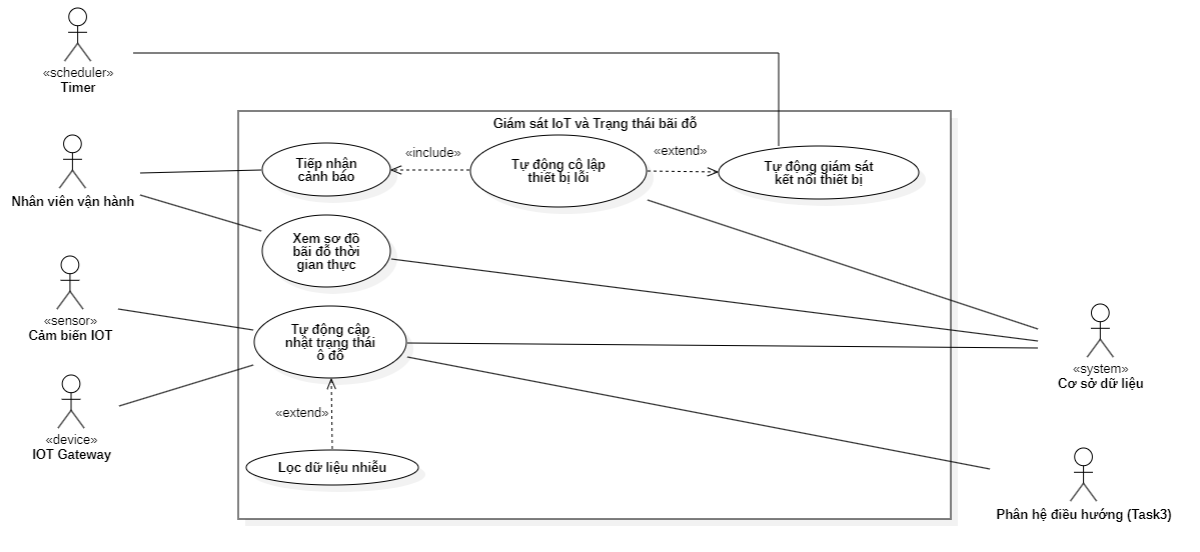
\includegraphics[width=1.2\textwidth]{pictures/UCD_Task2.png} 
    \caption{Use-case diagram cho Phân hệ Giám sát IoT và Trạng thái bãi đỗ}
    \label{UCD_2}
\end{figure}

\subsubsection{Use-case scenarios}
\noindent \textbf{Use Case: Xem sơ đồ bãi đỗ thời gian thực} \\
\renewcommand{\arraystretch}{1.6}
\begin{xltabular}{\textwidth}{|l|X|}
\hline
\textbf{Thuộc tính} & \textbf{Chi tiết} \\
\hline
\textbf{Tên} & Xem sơ đồ bãi đỗ thời gian thực \\
\hline
\textbf{Tác nhân} & Nhân viên vận hành \\
\hline
\textbf{Mô tả} & Cung cấp giao diện bản đồ 2D trực quan, cập nhật liên tục vị trí trống, có xe hoặc đang bảo trì cho người quản lý. \\
\hline
\textbf{Tiền điều kiện} & Nhân viên đã đăng nhập thành công vào hệ thống giám sát bãi xe. \\
\hline
\textbf{Luồng chính} & 
1. Nhân viên truy cập vào chức năng "Sơ đồ bãi đỗ" trên giao diện quản trị.

2. Hệ thống gửi yêu cầu truy xuất dữ liệu trạng thái hiện tại từ CSDL trung tâm.

3. Hệ thống hiển thị sơ đồ mặt bằng bãi xe với các mã màu quy định: Xanh (Trống), Đỏ (Có xe), Xám (Lỗi/Bảo trì).

4. Hệ thống duy trì kết nối thời gian thực (Socket/SignalR) để tự động làm mới giao diện ngay khi có thay đổi từ phía cảm biến.\\
\hline

\textbf{Luồng ngoại lệ} & 
\textbf{Mất kết nối máy chủ}: Giao diện hiển thị thông báo "Mất kết nối, đang thử lại...", giữ nguyên dữ liệu hiển thị cuối cùng trước khi mất mạng để tránh gián đoạn hoàn toàn.\\
\hline

\textbf{Hậu điều kiện} & Nhân viên nắm bắt được tình trạng lấp đầy của bãi xe để điều phối giao thông nội bộ. \\
\hline
\end{xltabular}

\noindent \textbf{Use Case: Tự động giám sát kết nối thiết bị} \\
\renewcommand{\arraystretch}{1.6}
\begin{xltabular}{\textwidth}{|l|X|}
\hline
\textbf{Thuộc tính} & \textbf{Chi tiết} \\
\hline
\textbf{Tên} & Tự động giám sát kết nối thiết bị  \\
\hline
\textbf{Tác nhân} & Bộ định thời (Timer) \\
\hline
\textbf{Mô tả} & Hệ thống định kỳ kiểm tra trạng thái hoạt động của các thiết bị phần cứng để phát hiện sự cố rớt mạng hoặc hỏng hóc. \\
\hline
\textbf{Tiền điều kiện} & Hệ thống máy chủ trung tâm đang trong trạng thái hoạt động. \\
\hline
\textbf{Luồng chính} & 
1. Bộ định thời (Timer) kích hoạt tiến trình kiểm tra sức khỏe thiết bị theo chu kỳ cấu hình (vd: mỗi 60 giây).

2. Máy chủ gửi các gói tin kiểm tra (Ping/Heartbeat) đến toàn bộ danh sách các IoT Gateway trong mạng.

3. Các Gateway nhận lệnh và phản hồi bản tin xác nhận trạng thái (Acknowledge) về Server.

4. Máy chủ cập nhật nhật ký hoạt động, đánh dấu các thiết bị là "Online".\\
\hline

\textbf{Luồng ngoại lệ} & 
\textbf{Thiết bị không phản hồi (Timeout)}: Nếu sau 3 lần thử mà Gateway không phản hồi, máy chủ chuyển trạng thái thiết bị sang "Offline" và kích hoạt kịch bản xử lý lỗi.\\
\hline

\textbf{Hậu điều kiện} & Trạng thái sức khỏe của toàn bộ hạ tầng IoT được cập nhật mới nhất. \\
\hline
\end{xltabular}

\noindent \textbf{Use Case: Tự động cô lập thiết bị lỗi} \\
\renewcommand{\arraystretch}{1.6}
\begin{xltabular}{\textwidth}{|l|X|}
\hline
\textbf{Thuộc tính} & \textbf{Chi tiết} \\
\hline
\textbf{Tên} & Tự động cô lập thiết bị lỗi  \\
\hline
\textbf{Tác nhân} & Không có \\
\hline
\textbf{Mô tả} & Tự động khoanh vùng các vị trí đỗ xe bị mất tín hiệu để tránh việc báo sai số liệu chỗ trống cho người dùng. \\
\hline
\textbf{Tiền điều kiện} & Hệ thống ghi nhận có thiết bị Gateway hoặc cụm cảm biến bị mất kết nối (Offline). \\
\hline
\textbf{Luồng chính} & 
1. Hệ thống xác định danh sách các ID ô đỗ được quản lý bởi thiết bị đang gặp sự cố.

2. Chuyển trạng thái của các ô đỗ này trong CSDL sang "Không xác định / Đang bảo trì" (Grey out).

3. Tự động khấu trừ số ô đỗ bị lỗi ra khỏi thuật toán tính tổng chỗ trống hiện có của bãi xe.

4. Khởi tạo và đẩy một thông báo cảnh báo (Alert) màu đỏ lên màn hình của Nhân viên vận hành.\\
\hline

\textbf{Luồng ngoại lệ} & 
\textbf{Tự phục hồi (Auto-recovery)}: Khi Timer phát hiện Gateway đã có tín hiệu trở lại, hệ thống yêu cầu Gateway gửi bản cập nhật trạng thái toàn phần để đồng bộ lại dữ liệu và đưa ô đỗ về trạng thái hoạt động.\\
\hline

\textbf{Hậu điều kiện} & Lỗi được cô lập an toàn, hệ thống điều hướng bảng LED không hiển thị số liệu sai lệch gây ùn tắc. \\
\hline
\end{xltabular}

\subsection{Điều hướng Giao thông}
\subsubsection{Tổng quan}
Phân hệ Điều hướng Giao thông đóng vai trò cốt lõi trong việc tối ưu hóa luồng phương tiện và nâng cao trải nghiệm của người dùng trong khuôn viên trường đại học. Dựa trên nguồn dữ liệu thời gian thực được luân chuyển từ phân hệ Giám sát IoT, hệ thống tự động phân tích tình trạng sức chứa của từng khu vực (còn chỗ, gần đầy, hoặc hết chỗ) để tính toán luồng di chuyển tối ưu. Các thông tin chỉ dẫn này sau đó được truyền tải liên tục thành các lệnh điều khiển động lên mạng lưới bảng hiển thị LED đặt tại các cổng và nút giao quan trọng, giúp tài xế nhanh chóng tìm được vị trí đỗ hoặc chuyển hướng sang các bãi xe thay thế. Đồng thời, phân hệ cung cấp giao diện quản lý để cấu hình vị trí bảng chỉ dẫn và phát đi các thông báo thủ công khi có sự kiện đặc biệt.

\subsubsection{Use-case diagram}
\begin{figure}[H]
    \centering
    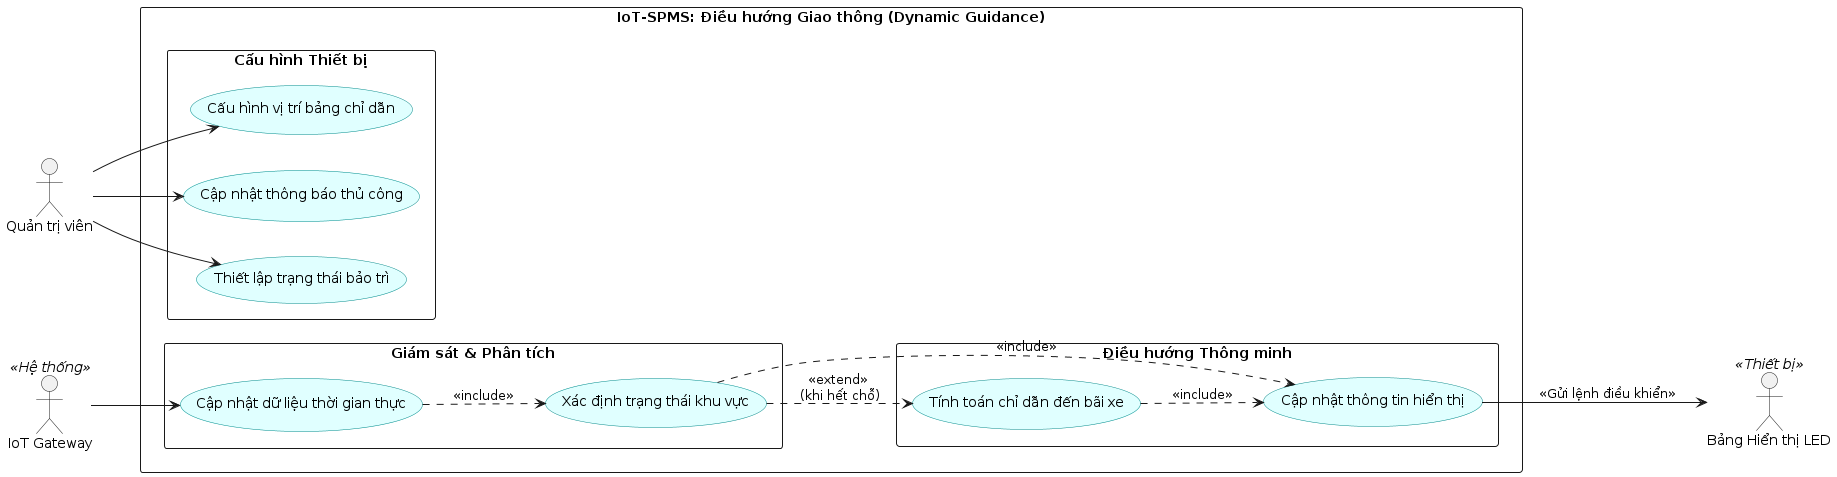
\includegraphics[width=1.15\textwidth]{pictures/task3_uc_diagram.png} 
    \caption{Use-case diagram cho Phân hệ Điều hướng giao thông}
    \label{UCD_3}
\end{figure}

\newpage
\subsubsection{Use-case scenarios}
\noindent \textbf{Use Case: Hiển thị trạng thái bãi đỗ xe} \\
\renewcommand{\arraystretch}{1.6}
\begin{xltabular}{\textwidth}{|l|X|}
\hline
\textbf{Thuộc tính} & \textbf{Chi tiết} \\
\hline
\textbf{Tên} & Hiển thị trạng thái bãi đỗ xe  \\
\hline
\textbf{Tác nhân} & Người lái xe (Sinh viên / Cán bộ / Khách), Bảng hiển thị LED \\
\hline
\textbf{Mô tả} & Hệ thống hiển thị trạng thái hiện tại của các khu vực bãi xe (Còn chỗ, Gần đầy, Hết chỗ) trên các bảng hiển thị điện tử đặt tại cổng hoặc các nút giao trong khuôn viên. \\
\hline
\textbf{Tiền điều kiện} & Hệ thống đã có dữ liệu trạng thái chỗ đậu xe được cập nhật từ các cảm biến thông qua IoT Gateway. \\
\hline
\textbf{Luồng chính} & 
1. Hệ thống thu thập dữ liệu trạng thái chỗ đậu xe từ cơ sở dữ liệu. 

2. Hệ thống tổng hợp số lượng chỗ trống của từng khu vực bãi xe. 

3. Hệ thống xác định trạng thái của từng khu vực (Còn chỗ / Gần đầy / Hết chỗ). 

4. Hệ thống gửi thông tin trạng thái tới các bảng hiển thị LED. 

5. Bảng hiển thị LED cập nhật và hiển thị thông tin cho người lái xe.
\\
\hline

\textbf{Luồng ngoại lệ} & 
\textbf{Dữ liệu cảm biến không đầy đủ}: hệ thống sử dụng dữ liệu gần nhất đã lưu và hiển thị trạng thái tạm thời. 

\textbf{Lỗi kết nối với bảng hiển thị}: hệ thống ghi log cảnh báo và thử gửi lại dữ liệu.
\\
\hline

\textbf{Hậu điều kiện} & Người lái xe có thể quan sát trạng thái bãi xe để quyết định hướng di chuyển. \\
\hline
\end{xltabular}

\noindent \textbf{Use Case: Điều hướng tới khu vực còn chỗ} \\
\renewcommand{\arraystretch}{1.6}
\begin{xltabular}{\textwidth}{|l|X|}
\hline
\textbf{Thuộc tính} & \textbf{Chi tiết} \\
\hline
\textbf{Tên} & Điều hướng tới khu vực còn chỗ  \\
\hline
\textbf{Tác nhân} & Người lái xe, Bảng hiển thị LED \\
\hline
\textbf{Mô tả} & Hệ thống phân tích trạng thái bãi xe và hiển thị hướng dẫn tới khu vực còn chỗ trống phù hợp thông qua bảng hiển thị điện tử. \\
\hline
\textbf{Tiền điều kiện} & Hệ thống đã có dữ liệu trạng thái chỗ đậu xe được cập nhật từ các cảm biến thông qua IoT Gateway. \\
\hline
\textbf{Luồng chính} & 
1. Người lái xe tiếp cận một nút giao hoặc cổng bãi xe. 

2. Hệ thống phân tích trạng thái các khu vực bãi xe. 

3. Hệ thống xác định khu vực còn nhiều chỗ trống hoặc gần nhất. 

4. Hệ thống tạo thông tin chỉ dẫn (mũi tên, tên bãi xe hoặc thông báo). 

5. Hệ thống gửi thông tin chỉ dẫn tới bảng hiển thị LED. 

6. Bảng hiển thị hiển thị hướng dẫn để người lái xe di chuyển tới khu vực phù hợp.
\\
\hline

\textbf{Luồng ngoại lệ} & 
\textbf{Tất cả bãi xe đều đầy}: hệ thống hiển thị thông báo “Bãi xe đã đầy”. 

\textbf{Dữ liệu trạng thái không đồng bộ}: hệ thống sử dụng dữ liệu gần nhất và ghi log cảnh báo.
\\
\hline

\textbf{Hậu điều kiện} & Người lái xe được hướng dẫn tới khu vực bãi xe còn chỗ. \\
\hline
\end{xltabular}

\noindent \textbf{Use Case: Cấu hình bảng hiển thị điện tử} \\
\renewcommand{\arraystretch}{1.6}
\begin{xltabular}{\textwidth}{|l|X|}
\hline
\textbf{Thuộc tính} & \textbf{Chi tiết} \\
\hline
\textbf{Tên} & Cấu hình bảng hiển thị điện tử  \\
\hline
\textbf{Tác nhân} & Quản trị viên (Admin) \\
\hline
\textbf{Mô tả} & Quản trị viên thiết lập hoặc chỉnh sửa cấu hình của các bảng hiển thị điện tử như vị trí, nội dung hiển thị hoặc trạng thái hoạt động. \\
\hline
\textbf{Tiền điều kiện} & Admin đã đăng nhập vào hệ thống quản trị và có quyền cấu hình thiết bị. \\
\hline
\textbf{Luồng chính} & 
1. Admin truy cập vào chức năng quản lý bảng hiển thị. 

2. Hệ thống hiển thị danh sách các bảng hiển thị hiện có. 

3. Admin chọn thêm mới hoặc chỉnh sửa cấu hình của một bảng hiển thị. 

4. Admin nhập các thông tin như vị trí, nội dung hiển thị hoặc trạng thái hoạt động. 

5. Admin lưu cấu hình. 

6. Hệ thống kiểm tra tính hợp lệ và lưu cấu hình vào cơ sở dữ liệu.
\\
\hline

\textbf{Luồng ngoại lệ} & 
\textbf{Thông tin cấu hình không hợp lệ}: hệ thống hiển thị thông báo lỗi và yêu cầu nhập lại. 

\textbf{Lỗi kết nối với thiết bị}: hệ thống ghi log cảnh báo và thông báo cho admin.
\\
\hline

\textbf{Hậu điều kiện} & Cấu hình bảng hiển thị được cập nhật và sẵn sàng sử dụng.\\
\hline
\end{xltabular}

\subsection{Quản lý Tính phí và Thanh toán}
\subsubsection{Tổng quan}
Phân hệ Quản lý Tính phí và Thanh toán đảm nhiệm việc tự động hóa toàn bộ quy trình tài chính liên quan đến hoạt động gửi xe trong khuôn viên trường. Phân hệ cung cấp các công cụ chuyên sâu để Quản trị viên cấu hình linh hoạt chính sách giá và quyền lợi đỗ xe cho từng nhóm đối tượng cụ thể (sinh viên, cán bộ, giảng viên). Thay vì thu phí thủ công từng lượt, hệ thống sẽ tự động tổng hợp các phiên gửi xe theo chu kỳ thời gian, tính toán chi phí phát sinh và cho phép người dùng khởi tạo yêu cầu thanh toán thông qua việc tích hợp trực tiếp với nền tảng BKPay. Nhờ cơ chế theo dõi nợ phí và cập nhật trạng thái giao dịch tự động qua Webhook/Callback, phân hệ này đảm bảo tính minh bạch, độ chính xác tuyệt đối và sự tiện lợi tối đa trong công tác đối soát tài chính.

\subsubsection{Use-case diagram}
\begin{figure}[H]
    \centering
    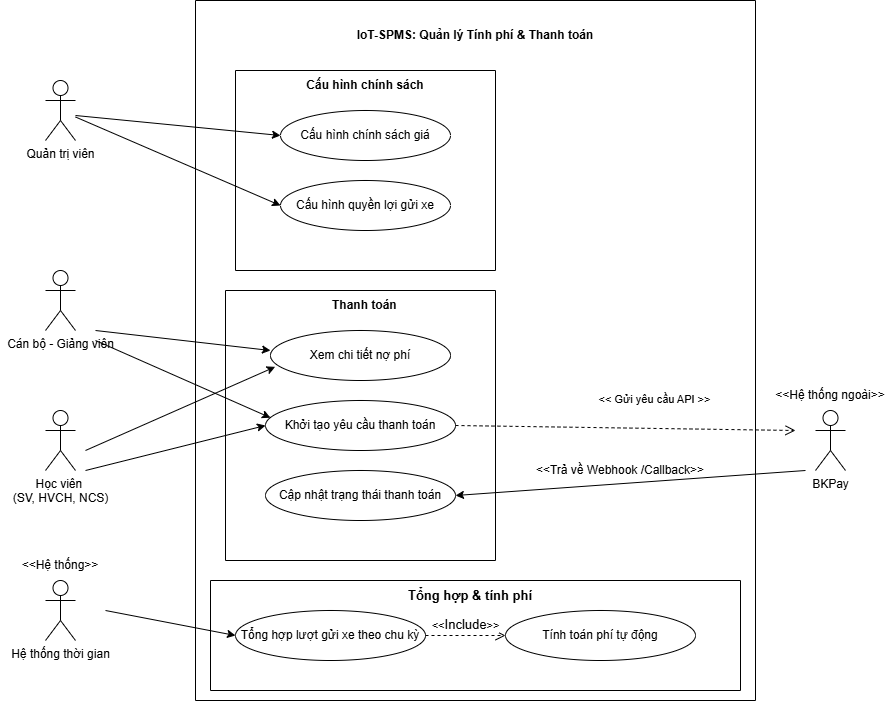
\includegraphics[width=1.15\textwidth]{pictures/UCD_Task4.jpg} 
    \caption{Use-case diagram cho Phân hệ Quản lý Tính phí và thanh toán}
    \label{UCD_4}
\end{figure}

\subsubsection{Use-case scenarios}

\noindent \textbf{Use Case: Cấu hình chính sách giá} \\
\renewcommand{\arraystretch}{1.6}
\begin{xltabular}{\textwidth}{|l|X|}
\hline
\textbf{Thuộc tính} & \textbf{Chi tiết} \\
\hline
\textbf{Tên} & Cấu hình chính sách giá \\
\hline
\textbf{Tác nhân} & Quản trị viên (Admin) \\
\hline
\textbf{Mô tả} & Cho phép quản trị viên thiết lập, chỉnh sửa bảng giá gửi xe áp dụng cho từng nhóm đối tượng (Người học, Giảng viên, Khách) theo từng khung giờ hoặc loại phương tiện. \\
\hline
\textbf{Tiền điều kiện} & Admin đã đăng nhập thành công qua HCMUT\_SSO và có quyền quản trị tài chính. \\
\hline
\textbf{Luồng chính} & 
1. Admin chọn chức năng "Quản lý chính sách giá".

2. Hệ thống hiển thị danh sách các chính sách hiện tại.

3. Admin chọn thêm mới hoặc chỉnh sửa một chính sách (vd: Phí tháng cho SV).

4. Admin nhập các thông số: Loại người dùng, mức giá, thời gian áp dụng.

5. Admin nhấn "Lưu".

6. Hệ thống kiểm tra tính hợp lệ của dữ liệu, lưu vào cơ sở dữ liệu và hiển thị thông báo thành công.
\\
\hline

\textbf{Luồng ngoại lệ} & 
\textbf{Dữ liệu không hợp lệ}: Hệ thống cảnh báo các trường thông tin sai định dạng (vd: giá trị âm) và yêu cầu nhập lại.

\textbf{Trùng lặp khoảng thời gian}: Cảnh báo chính sách mới chồng chéo thời gian với chính sách cũ.
\\
\hline

\textbf{Hậu điều kiện} & Bảng giá mới được lưu trữ và sẵn sàng áp dụng cho các lượt tính toán phí tiếp theo.\\
\hline
\end{xltabular}

\noindent \textbf{Use Case: Tổng hợp và tính toán chi phí tự động} \\
\renewcommand{\arraystretch}{1.6}
\begin{xltabular}{\textwidth}{|l|X|}
\hline
\textbf{Thuộc tính} & \textbf{Chi tiết} \\
\hline
\textbf{Tên} & Tổng hợp và tính toán chi phí tự động \\
\hline
\textbf{Tác nhân} & Hệ thống thời gian (Time-triggered System) \\
\hline
\textbf{Mô tả} & Hệ thống tự động gom nhóm các lượt ra/vào của người dùng theo chu kỳ (ví dụ: cuối tháng) và áp dụng chính sách giá để ra tổng số tiền cần thanh toán. \\
\hline
\textbf{Tiền điều kiện} & Đến thời điểm chốt chu kỳ thanh toán đã được cấu hình trước; Dữ liệu log gửi xe đầy đủ. \\
\hline
\textbf{Luồng chính} & 
1. Tới thời điểm cấu hình (vd: 23:59 ngày cuối tháng), hệ thống kích hoạt tiến trình chạy ngầm (batch job).

2. Truy xuất toàn bộ log ra/vào trong chu kỳ của từng thẻ định danh.

3. Kiểm tra thông tin chức danh (Role) từ dữ liệu HCMUT\_DATACORE.

4. Đối chiếu với "Chính sách giá" và "Quyền lợi" tương ứng.

5. Tính tổng số tiền phát sinh cho từng người dùng.

6. Tạo bản ghi hóa đơn (Billing Record) với trạng thái "Chưa thanh toán".
\\
\hline

\textbf{Luồng ngoại lệ} & 
\textbf{Lỗi thiếu dữ liệu thẻ}: Ghi log lỗi vào hệ thống giám sát cảnh báo Admin, bỏ qua bản ghi lỗi và tiếp tục xử lý các bản ghi khác để không dừng toàn bộ tiến trình.
\\
\hline

\textbf{Hậu điều kiện} & Cơ sở dữ liệu xuất hiện các bản ghi hóa đơn mới. Người dùng có thể xem được khoản nợ của mình.\\
\hline
\end{xltabular}

\noindent \textbf{Use Case: Khởi tạo yêu cầu thanh toán qua BKPay} \\
\renewcommand{\arraystretch}{1.6}
\begin{xltabular}{\textwidth}{|l|X|}
\hline
\textbf{Thuộc tính} & \textbf{Chi tiết} \\
\hline
\textbf{Tên} & Khởi tạo yêu cầu thanh toán qua BKPay \\
\hline
\textbf{Tác nhân} & Thành viên trường, Hệ thống BKPay \\
\hline
\textbf{Mô tả} & Người dùng thực hiện thanh toán khoản phí gửi xe định kỳ thông qua cổng thanh toán BKPay của trường. \\
\hline
\textbf{Tiền điều kiện} & Người dùng có hóa đơn ở trạng thái "Chưa thanh toán"; BKPay đang hoạt động bình thường. \\
\hline
\textbf{Luồng chính} & 
1. Người dùng đăng nhập portal, vào mục "Thanh toán phí gửi xe".

2. Hệ thống hiển thị chi tiết hóa đơn chu kỳ.

3. Người dùng chọn "Thanh toán qua BKPay".

4. IoT-SPMS mã hóa thông tin hóa đơn và gọi API khởi tạo giao dịch sang BKPay.

5. Hệ thống chuyển hướng (redirect) người dùng sang giao diện BKPay.

6. Người dùng thao tác thanh toán trên BKPay (nhập thẻ, quét QR...).

7. BKPay gọi API Webhook trả về trạng thái giao dịch thành công cho IoT-SPMS.

8. IoT-SPMS cập nhật trạng thái hóa đơn thành "Đã thanh toán".
\\
\hline

\textbf{Luồng ngoại lệ} & 
\textbf{EF1: Giao dịch thất bại / Hủy bỏ}: BKPay trả về trạng thái lỗi. IoT-SPMS giữ nguyên trạng thái hóa đơn, hiển thị thông báo "Thanh toán thất bại" cho người dùng.\newline
\textbf{EF2: Mất kết nối API}: IoT-SPMS không gọi được BKPay, hiển thị thông báo "Cổng thanh toán đang bảo trì".
\\
\hline

\textbf{Hậu điều kiện} & Hóa đơn được cập nhật trạng thái chuẩn xác. Số dư/khoản nợ của người dùng được khấu trừ.\\
\hline
\end{xltabular}

\newpage
\noindent \textbf{Use Case: Xem hóa đơn và lịch sử giao dịch} \\
\renewcommand{\arraystretch}{1.6}
\begin{xltabular}{\textwidth}{|l|X|}
\hline
\textbf{Thuộc tính} & \textbf{Chi tiết} \\
\hline
\textbf{Tên} & Xem hóa đơn và lịch sử giao dịch \\
\hline
\textbf{Tác nhân} & Thành viên trường \\
\hline
\textbf{Mô tả} & Người dùng tra cứu hóa đơn hiện tại theo chu kỳ và xem danh sách giao dịch thanh toán đã phát sinh (thành công/thất bại). \\
\hline
\textbf{Tiền điều kiện} & Người dùng đã đăng nhập; hệ thống đã tạo Billing Record (nếu đến kỳ chốt) hoặc có dữ liệu giao dịch trước đó. \\
\hline
\textbf{Luồng chính} &
1. Người dùng truy cập mục "Pricing/Hóa đơn".

2. Hệ thống hiển thị hóa đơn gần nhất (mã hóa đơn, chu kỳ, số tiền, trạng thái) và nút thao tác (Thanh toán/Làm mới).

3. Người dùng chuyển sang tab "Giao dịch".

4. Hệ thống hiển thị danh sách các giao dịch theo thời gian (mã giao dịch, số tiền, trạng thái, thời điểm).
\\
\hline

\textbf{Luồng ngoại lệ} &
\textbf{Không có hóa đơn/giao dịch}: Hệ thống hiển thị thông báo "Chưa có dữ liệu" và ẩn các thao tác không phù hợp.
\\
\hline

\textbf{Hậu điều kiện} & Người dùng nắm được khoản phí cần thanh toán và trạng thái giao dịch phục vụ đối soát cá nhân.\\
\hline
\end{xltabular}

\newpage
\noindent \textbf{Use Case: Xử lý Webhook/Callback từ BKPay} \\
\renewcommand{\arraystretch}{1.6}
\begin{xltabular}{\textwidth}{|l|X|}
\hline
\textbf{Thuộc tính} & \textbf{Chi tiết} \\
\hline
\textbf{Tên} & Xử lý Webhook/Callback từ BKPay \\
\hline
\textbf{Tác nhân} & Hệ thống BKPay \\
\hline
\textbf{Mô tả} & BKPay gửi thông báo bất đồng bộ (webhook/callback) về kết quả giao dịch để IoT-SPMS cập nhật trạng thái hóa đơn và giao dịch. \\
\hline
\textbf{Tiền điều kiện} & Một giao dịch đã được khởi tạo; endpoint webhook của IoT-SPMS sẵn sàng; BKPay có khả năng ký/đính kèm HMAC. \\
\hline
\textbf{Luồng chính} &
1. BKPay gửi webhook chứa: mã giao dịch, mã hóa đơn, trạng thái (SUCCESS/FAILED/CANCELED), thời gian, chữ ký (HMAC).

2. IoT-SPMS kiểm tra tính toàn vẹn (verify HMAC) và kiểm tra tính hợp lệ (invoiceId/txId tồn tại).

3. IoT-SPMS áp dụng cơ chế idempotency: nếu webhook trùng lặp, hệ thống không cập nhật lại trạng thái đã chốt.

4. Nếu trạng thái SUCCESS: cập nhật giao dịch "Thành công" và hóa đơn "Đã thanh toán" (ghi nhận paidAt).

5. Ghi log/audit trail phục vụ đối soát.
\\
\hline

\textbf{Luồng ngoại lệ} &
\textbf{EF1: Chữ ký không hợp lệ}: Từ chối xử lý, trả mã lỗi; ghi log cảnh báo bảo mật.\newline
\textbf{EF2: Thiếu dữ liệu / không tìm thấy hóa đơn}: Trả lỗi và ghi log; không thay đổi dữ liệu.\newline
\textbf{EF3: Lỗi CSDL khi cập nhật}: Rollback transaction và trả lỗi để BKPay retry.
\\
\hline

\textbf{Hậu điều kiện} & Trạng thái hóa đơn/giao dịch được đồng bộ chuẩn xác với BKPay và có thể truy vết.\\
\hline
\end{xltabular}

\subsection{Các yêu cầu chức năng phi tương tác}
\subsubsection{Tổng quan}
Hệ thống bao gồm một số quy trình nền không tương tác, chạy tự động để đảm bảo tính toàn vẹn dữ liệu, liên lạc kịp thời và kiểm soát truy cập phù hợp. Các trường hợp sử dụng này được kích hoạt bởi các sự kiện hệ thống hoặc các tác vụ theo lịch trình (cron jobs) và không yêu cầu người dùng tương tác trực tiếp để thực thi. Chúng rất cần thiết cho việc tự động hóa và tăng độ tin cậy của Hệ thống Quản lý Bãi đỗ xe thông minh.

\subsubsection{Use-case diagram}
\begin{figure}[H]
    \centering
    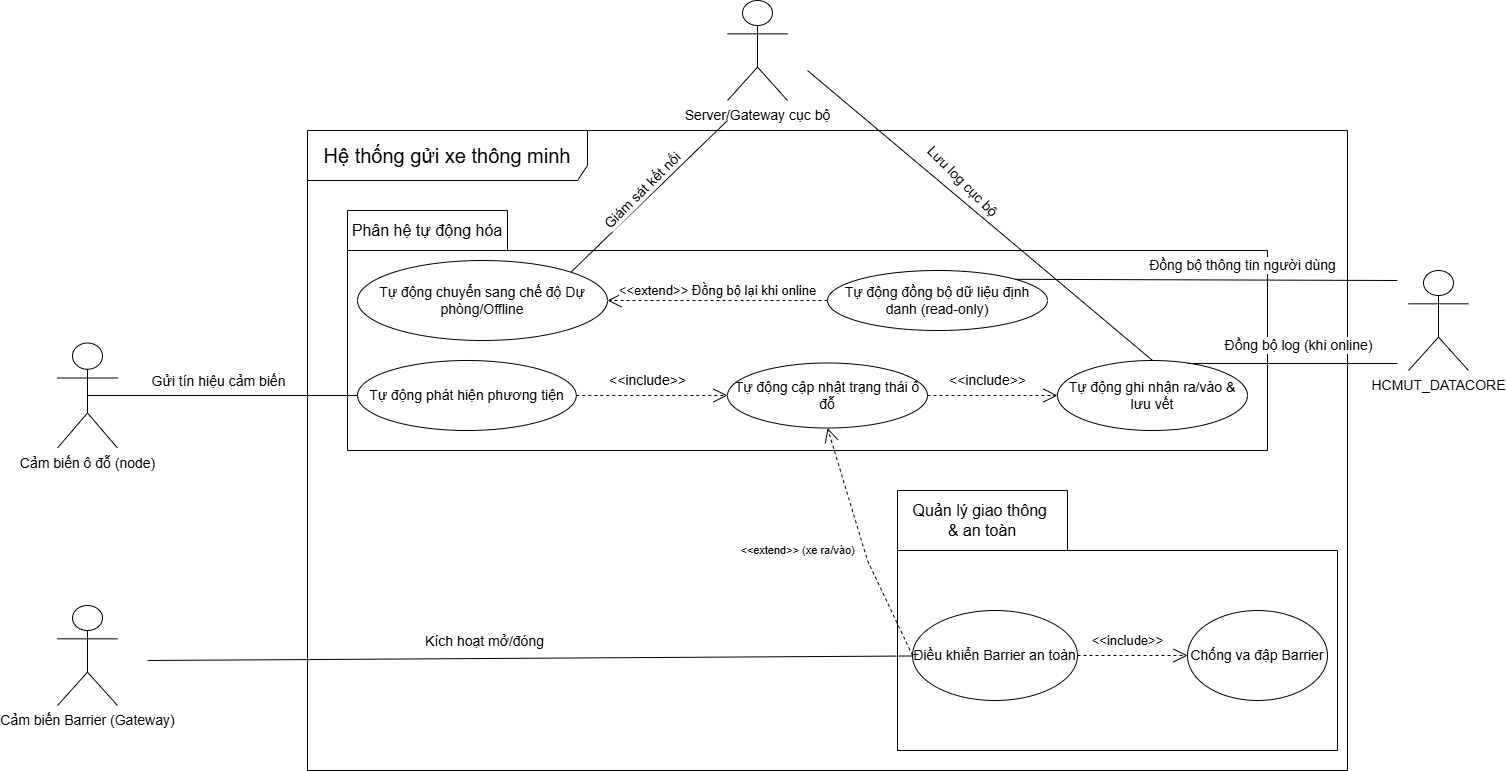
\includegraphics[width=1.15\textwidth]{pictures/se_nonin.drawio.png} 
    \caption{Use-case diagram cho Yêu cầu chức năng phi tương tác thứ 1}
    \label{UCD_n-i_1}
\end{figure}

\subsubsection{Use-case scenarios}
\newpage
\noindent \textbf{Use Case: Tự động đồng bộ dữ liệu} \\
\renewcommand{\arraystretch}{1.6}
\begin{xltabular}{\textwidth}{|l|X|}
\hline
\textbf{Thuộc tính} & \textbf{Chi tiết} \\
\hline
\textbf{Tên} & Tự động đồng bộ dữ liệu \\
\hline
\textbf{Tác nhân} & Timer (Bộ định thời), HCMUT\_DATACORE \\
\hline
\textbf{Mô tả} & Hệ thống Gateway định kỳ tải về danh sách định danh hợp lệ từ server trung tâm mà không cần người dùng can thiệp. \\
\hline
\textbf{Tiền điều kiện} & Hệ thống Gateway nội bộ có kết nối mạng Internet ổn định tới HCMUT\_DATACORE. \\
\hline
\textbf{Luồng chính} & 
1. Bộ định thời (Timer) trên Gateway kích hoạt sự kiện đồng bộ theo chu kỳ (ví dụ: mỗi 30 phút).


2. Gateway gửi HTTP GET Request (chỉ đọc) đến API của HCMUT\_DATACORE.


3. Hệ thống nhận payload JSON chứa danh sách ID thẻ và quyền truy cập mới nhất.


4. Gateway tiến hành cập nhật/ghi đè các bản ghi thay đổi vào cơ sở dữ liệu cục bộ (Local Cache / SQLite).


5. Hệ thống ghi log hoàn tất tiến trình đồng bộ.
\\
\hline

\textbf{Luồng ngoại lệ} & 
\textbf{Mất kết nối API / Timeout}: Hệ thống ghi log lỗi (Error log), giữ nguyên cơ sở dữ liệu cache cũ để đảm bảo tính sẵn sàng và chờ đến chu kỳ đồng bộ tiếp theo.
\\
\hline

\textbf{Hậu điều kiện} & Dữ liệu định danh tại Gateway cục bộ được làm mới, khớp với dữ liệu trung tâm.\\
\hline
\end{xltabular}

\noindent \textbf{Use Case: Tự động cập nhật trạng thái bãi đỗ} \\
\renewcommand{\arraystretch}{1.6}
\begin{xltabular}{\textwidth}{|l|X|}
\hline
\textbf{Thuộc tính} & \textbf{Chi tiết} \\
\hline
\textbf{Tên} & Tự động cập nhật trạng thái bãi đỗ \\
\hline
\textbf{Tác nhân} & Cảm biến IoT \\
\hline
\textbf{Mô tả} & Hệ thống tự động nhận diện xe ra/vào từng ô đỗ và tính toán lại tổng số chỗ trống của toàn bãi. \\
\hline
\textbf{Tiền điều kiện} & Các Node cảm biến (VD: ESP32 gắn cảm biến siêu âm) đang hoạt động và kết nối vào mạng nội bộ. \\
\hline
\textbf{Luồng chính} & 
1. Cảm biến tại ô đỗ phát hiện sự thay đổi trạng thái (từ "trống" sang "có xe" hoặc ngược lại).

2. Node cảm biến đóng gói dữ liệu và gửi bản tin qua giao thức truyền thông (ví dụ: MQTT) về bộ điều khiển Gateway.

3. Hệ thống xử lý bản tin và tự động cộng/trừ số lượng chỗ trống tương ứng.

4. Hệ thống xuất lệnh điều khiển gửi xuống bảng LED ma trận tại cổng để cập nhật con số hiển thị mới nhất.

5. Dữ liệu trạng thái được đẩy lên server trung tâm.
\\
\hline

\textbf{Luồng ngoại lệ} & 
\textbf{Cảm biến hỏng / Mất tín hiệu}: Nếu Gateway không nhận được tín hiệu "heartbeat" từ một Node quá thời gian quy định, hệ thống tự động đánh dấu ô đỗ đó là "Bảo trì" và báo cáo cho Nhân viên vận hành.
\\
\hline

\textbf{Hậu điều kiện} & Trạng thái bãi đỗ (trên phần mềm và bảng LED) hiển thị chính xác số chỗ trống thực tế.\\
\hline
\end{xltabular}

\noindent \textbf{Use Case: Tự động đóng barrier an toàn} \\
\renewcommand{\arraystretch}{1.6}
\begin{xltabular}{\textwidth}{|l|X|}
\hline
\textbf{Thuộc tính} & \textbf{Chi tiết} \\
\hline
\textbf{Tên} & Tự động đóng barrier an toàn \\
\hline
\textbf{Tác nhân} & Cảm biến IoT (Vòng từ Loop Detector / Cảm biến quang) \\
\hline
\textbf{Mô tả} & Chức năng tự động hóa phần cứng giúp barrier nhận biết chính xác thời điểm xe đã đi qua cổng hoàn toàn. \\
\hline
\textbf{Tiền điều kiện} & Barrier đang ở trạng thái mở (đã xác thực thành công). Xe đang di chuyển qua cổng. \\
\hline
\textbf{Luồng chính} & 
1. Phương tiện di chuyển qua cổng, cắt ngang vùng phát hiện của cảm biến quang hoặc đè lên vòng từ.

2. Khi xe đã đi qua hoàn toàn, cảm biến gửi tín hiệu ngắt (interrupt) về bo mạch điều khiển cổng.

3. Bo mạch xác nhận vùng an toàn dưới barrier không còn chướng ngại vật.

4. Hệ thống kích hoạt Relay để hạ cần barrier xuống.

5. Ghi nhận thời gian đóng barrier vào log hệ thống.
\\
\hline

\textbf{Luồng ngoại lệ} & 
\textbf{Có vật cản mắc kẹt}: Nếu xe dừng lại hoặc có người đứng ngay dưới barrier, cảm biến liên tục gửi tín hiệu có chướng ngại vật. Hệ thống từ chối lệnh đóng và giữ nguyên barrier ở trạng thái mở để chống va đập.
\\
\hline

\textbf{Hậu điều kiện} & Barrier được đóng lại an toàn, luồng giao thông tại cổng được khóa chặt chờ phiên tiếp theo.\\
\hline
\end{xltabular}


\noindent \textbf{Use Case: Tự động chuyển đổi cơ chế dự phòng} \\
\renewcommand{\arraystretch}{1.6}
\begin{xltabular}{\textwidth}{|l|X|}
\hline
\textbf{Thuộc tính} & \textbf{Chi tiết} \\
\hline
\textbf{Tên} & Tự động chuyển đổi cơ chế dự phòng \\
\hline
\textbf{Tác nhân} & Timer (Bộ định thời) \\
\hline
\textbf{Mô tả} & Hệ thống theo dõi liên tục trạng thái kết nối và tự động kích hoạt chế độ ngoại tuyến (Offline) khi phát hiện sự cố. \\
\hline
\textbf{Tiền điều kiện} & Hệ thống đang ở trạng thái Online. Local Cache đã có dữ liệu thẻ. \\
\hline
\textbf{Luồng chính} & 
1. Bộ định thời của hệ thống liên tục gửi các gói tin Heartbeat/Ping đến máy chủ HCMUT\_SSO.

2. Hệ thống phát hiện không nhận được phản hồi (Timeout) sau 3 lần thử liên tiếp.

3. Hệ thống tự động thay đổi cờ trạng thái mạng sang "Offline".

4. Hệ thống chuyển hướng toàn bộ các truy vấn xác thực thẻ tiếp theo xuống cơ sở dữ liệu cục bộ.

5. Bảng LED tại cổng hiển thị dòng chữ cảnh báo nhỏ "Chế độ ngoại tuyến".
\\
\hline

\textbf{Luồng ngoại lệ} & 
\textbf{Khi có mạng trở lại}: Timer phát hiện tín hiệu Ping thành công. Hệ thống tự động chuyển về trạng thái Online và tiến hành chạy ngầm tiến trình đẩy (push) toàn bộ log các lượt gửi xe ngoại tuyến lên server trung tâm.
\\
\hline

\textbf{Hậu điều kiện} & Hệ thống hoạt động độc lập an toàn, hoạt động kiểm tra thẻ không bị gián đoạn.\\
\hline
\end{xltabular}


\subsubsection{Use-case diagram}
\begin{figure}[H]
    \centering
    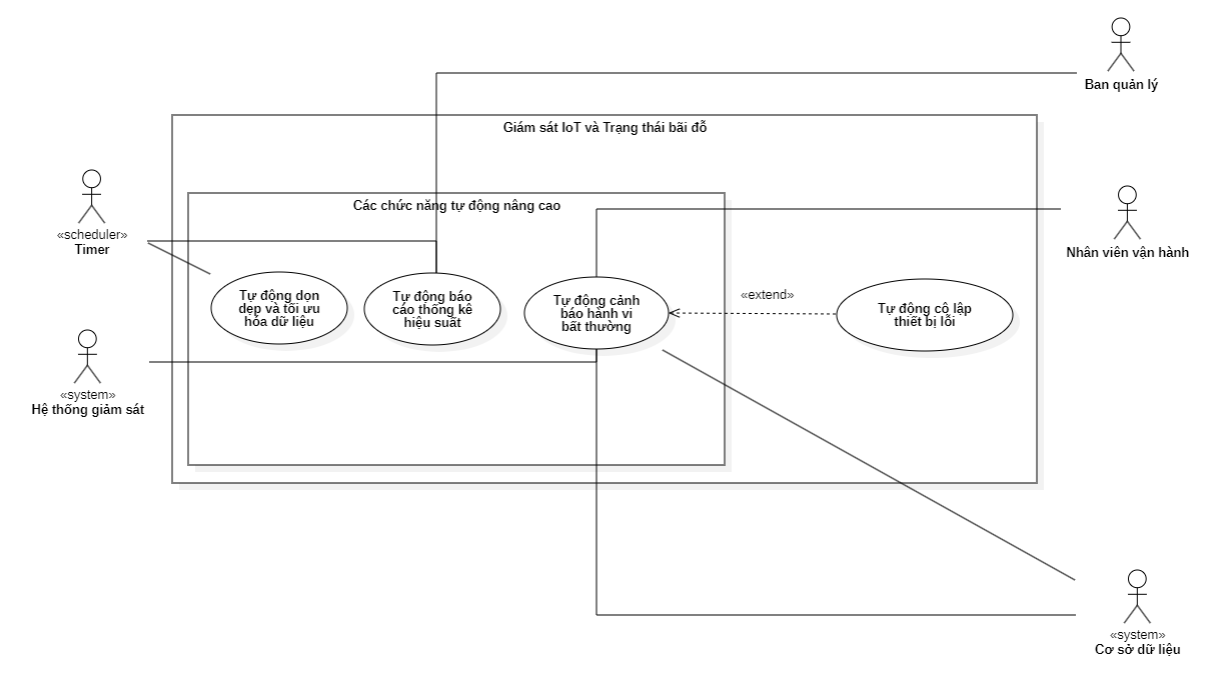
\includegraphics[width=1.15\textwidth]{pictures/non_in2.png} 
    \caption{Use-case diagram cho Yêu cầu chức năng phi tương tác thứ 2}
    \label{UCD_n-i_2}
\end{figure}

\subsubsection{Use-case scenarios}

\noindent \textbf{Use Case: Tự động dọn dẹp và tối ưu hóa dữ liệu} \\
\renewcommand{\arraystretch}{1.6}
\begin{xltabular}{\textwidth}{|l|X|}
\hline
\textbf{Thuộc tính} & \textbf{Chi tiết} \\
\hline
\textbf{Tên} & Tự động dọn dẹp và tối ưu hóa dữ liệu \\
\hline
\textbf{Tác nhân} & Timer (Bộ định thời) \\
\hline
\textbf{Mô tả} & Tự động xóa các bản ghi log trạng thái quá hạn để tránh làm đầy bộ nhớ của thiết bị Gateway cục bộ. \\
\hline
\textbf{Tiền điều kiện} & Hệ thống Gateway đang hoạt động và có quyền truy cập vào CSDL cục bộ. \\
\hline
\textbf{Luồng chính} & 
1. Đến giờ thấp điểm (vd: 02:00 AM), Timer kích hoạt tiến trình dọn dẹp.

2. Hệ thống thực hiện sao lưu các log quan trọng về Server trung tâm.

3. Hệ thống thực hiện lệnh xóa các log cũ (trên 7 ngày) tại bộ nhớ đệm của Gateway cục bộ.
\\
\hline

\textbf{Luồng ngoại lệ} & 
\textbf{Lỗi cấp quyền (Permission Denied)}: Nếu hệ thống không thể xóa file log do ổ cứng bị khóa, hệ thống sẽ ghi nhận cảnh báo vào Error Log và tự động thử lại vào chu kỳ của ngày hôm sau để không làm treo Gateway.
\\
\hline

\textbf{Hậu điều kiện} & Bộ nhớ thiết bị được giải phóng, duy trì hiệu năng hoạt động ổn định.\\
\hline
\end{xltabular}

\newpage
\noindent \textbf{Use Case: Tự động báo cáo thống kê hiệu suất} \\
\renewcommand{\arraystretch}{1.6}
\begin{xltabular}{\textwidth}{|l|X|}
\hline
\textbf{Thuộc tính} & \textbf{Chi tiết} \\
\hline
\textbf{Tên} & Tự động báo cáo thống kê hiệu suất \\
\hline
\textbf{Tác nhân} & Timer (Bộ định thời) \\
\hline
\textbf{Mô tả} & Cuối mỗi ngày, hệ thống tự động tính toán tỷ lệ lấp đầy bãi xe và gửi báo cáo tóm tắt cho ban quản lý. \\
\hline
\textbf{Tiền điều kiện} & CSDL trung tâm có lưu trữ đầy đủ nhật ký đỗ xe trong ngày. \\
\hline
\textbf{Luồng chính} & 
1. Đến 23:59 hàng ngày, Timer kích hoạt tiến trình tổng hợp số liệu.

2. Hệ thống thống kê tổng số lượt xe vào/ra và thời gian đỗ trung bình.

3. Hệ thống tính toán "Tỷ lệ lấp đầy cao nhất" trong ngày.

4. Tự động xuất file báo cáo (PDF/Excel) và gửi vào email của Ban quản lý.
\\
\hline

\textbf{Luồng ngoại lệ} & 
\textbf{Lỗi gửi Email (SMTP Error)}: Nếu máy chủ Mail bị lỗi không thể gửi đi, hệ thống sẽ lưu trữ file báo cáo tại thư mục cục bộ và hiển thị thông báo nhắc nhở lên màn hình Admin để quản lý tải về thủ công.
\\
\hline

\textbf{Hậu điều kiện} & Ban quản lý nhận được báo cáo tự động mà không cần tính toán thủ công.\\
\hline
\end{xltabular}

\noindent \textbf{Use Case: Tự động cảnh báo hành vi bất thường} \\
\renewcommand{\arraystretch}{1.6}
\begin{xltabular}{\textwidth}{|l|X|}
\hline
\textbf{Thuộc tính} & \textbf{Chi tiết} \\
\hline
\textbf{Tên} & Tự động cảnh báo hành vi bất thường \\
\hline
\textbf{Tác nhân} & Hệ thống \\
\hline
\textbf{Mô tả} & Tự động nhận diện các mẫu tín hiệu lỗi (nhảy trạng thái liên tục) để cảnh báo nguy cơ hỏng cảm biến hoặc có người phá hoại. \\
\hline
\textbf{Tiền điều kiện} & Cảm biến đang liên tục gửi dữ liệu về máy chủ. \\
\hline
\textbf{Luồng chính} & 
1. Hệ thống giám sát tần suất thay đổi trạng thái của từng ô đỗ.

2. Nếu một ô đỗ thay đổi trạng thái (Trống <-> Có xe) liên tục hơn 10 lần trong 1 phút, hệ thống xác định đây là tín hiệu nhiễu/lỗi.

3. Tự động khóa trạng thái ô đỗ đó để không làm sai lệch số liệu chỗ trống.

4. Phát thông báo khẩn cấp (Alert) cho Nhân viên vận hành để kiểm tra.
\\
\hline

\textbf{Luồng ngoại lệ} & 
\textbf{Cảm biến mất kết nối}: Nếu trong quá trình nhảy trạng thái liên tục mà cảm biến đột ngột mất tín hiệu hoàn toàn, hệ thống lập tức dừng kịch bản này và chuyển sang kích hoạt Kịch bản (Cô lập thiết bị lỗi).
\\
\hline

\textbf{Hậu điều kiện} & Ngăn chặn dữ liệu rác làm sai lệch hệ thống và phát hiện sớm hư hỏng phần cứng.\\
\hline
\end{xltabular}

